% !TEX program = lualatex
%==============================================================================
% プリアンブル (Preamble)
%==============================================================================

% ===== ドキュメントクラス =====
\documentclass[
    a4paper,
    11pt
]{ltjsreport}

%------------------------------------------------------------------------------
% パッケージ読み込み
%------------------------------------------------------------------------------

% ===== フォント・言語設定 (LuaLaTeX専用) =====
\usepackage{luatexja-fontspec}
\usepackage{lmodern} % フォントサイズの置き換えを防ぐため

% ===== レイアウト関連 =====
\usepackage[margin=2.5cm]{geometry}
\usepackage{booktabs}
\usepackage{float}
\usepackage{graphicx} % 画像挿入のために追加

% ===== 数式・物理単位関連 =====
\usepackage{amsmath}
\usepackage{siunitx}
\usepackage{bm} % ベクトルを太字にするため (\bm)

% ===== その他 =====
\usepackage{url} % URLを適切に表示
\urlstyle{same}
\Urlmuskip=0mu plus 1mu
\usepackage[
  colorlinks=true,
  linkcolor=blue,
  citecolor=green!60!black,
  urlcolor=cyan,
  hidelinks,
]{hyperref}

%------------------------------------------------------------------------------
% 各種設定
%------------------------------------------------------------------------------

% ===== フォント設定 =====
\setmainfont{Latin Modern Roman}
\setsansfont{Latin Modern Sans}
\setmonofont{Latin Modern Mono}
\setmainjfont[Renderer=HarfBuzz]{Yu Mincho}
\setsansjfont[Renderer=HarfBuzz]{Yu Gothic}
\DeclareMathSizes{11}{11}{7}{5} % 数学フォントサイズの調整

% ===== ドキュメント情報 =====
\title{高周波基板の損失測定に関する体系的知識の構築:\\
物理的原理から測定技術,損失分離まで}
\author{(氏名)}
\date{\today}

% ===== 数式用カスタムコマンド =====
\newcommand{\dd}{\mathrm{d}} % 微分演算子 d
\newcommand{\mi}{\mathrm{j}} % 虚数単位 j

%==============================================================================
% ドキュメント本体 (Body)
%==============================================================================
\begin{document}

\maketitle
\tableofcontents
\clearpage

% ===================================================================
\chapter*{序論:研究の核心的課題 — 「損失の分離」}
\addcontentsline{toc}{chapter}{序論:研究の核心的課題 — 「損失の分離」}
% ===================================================================

柳原さん,あなたの研究発表資料\cite{Yanagihara2025}を拝見しました.「BCDRを用いた基板の誘電損失と表面粗さによる電気伝導性の測定」という研究テーマは,\SI{100}{\giga\hertz}級の通信\cite{Yanagihara2025}を支える高周波工学において,最も本質的かつ重要な課題の一つである「損失の分離(Loss Separation)」に正面から取り組むものです.

あなたの発表資料\cite{Yanagihara2025}に示された2つの基本式,
\begin{align}
  \alpha &= \alpha_c + \alpha_d \label{eq:alpha_sum} \\
  \frac{1}{Q} &= \frac{1}{Q_c} + \frac{1}{Q_d} \label{eq:q_sum}
\end{align}
は,この「損失分離」の根幹を成します.ここで $\alpha$ は空間的な減衰(1メートル進むごとにどれだけ信号が弱まるか),$Q$ は時間的な減衰(共振器内でエネルギーがどれだけ長く留まるか)を表しており,両者は物理的に深く結びついています.

あなたの研究の最終目的は,導体損失 $\alpha_c$(あるいは $Q_c$)に対する「表面粗さ」の影響を明らかにすることです\cite{Yanagihara2025}.しかし,VNA(ベクトルネットワークアナライザ)で測定できるのは,常に「全体の損失 $\alpha$」あるいは「全体のQ値 $Q$」でしかありません.

したがって,あなたの研究の論理構造は,必然的に以下のようになります\cite{Yanagihara2025}.
\begin{enumerate}
  \item \textbf{目的:} $\alpha_c$(表面粗さを含む導体損失)を知りたい.
  \item \textbf{課題:} しかし測定できるのは $\alpha = \alpha_c + \alpha_d$(全体損失)だけであり,$\alpha_c$ と $\alpha_d$ は共に未知数である.
  \item \textbf{解決策:} 2つの未知数を分離するため,まず表面粗さの影響を排除した「基準系」で $\alpha_d$(誘電損失)を精密に決定する.次に,その既知の $\alpha_d$ を用いて,本測定系から $\alpha_c$ を正確に差し引く必要がある.
  \item \textbf{今回のアプローチ:} そこで,まずBCDR法という高感度な手法を用いて,$\alpha_d$(誘電損失,すなわち $\tan\delta$ や $Q_d$)を精密に測定することから始める\cite{Yanagihara2025}.
\end{enumerate}

本レポートは,この論理的なストーリーラインを物理的な本質から支えるための専門知識を体系的に解説するものです.第1部で損失の「物理的起源」,第2部でその「高感度測定と分離の原理」を詳述します.これらを修得することで,第3部の質疑応答に自信を持って臨むことができるでしょう.

\clearpage
% ===================================================================
\part{高周波における損失の物理}
% ===================================================================
高周波信号が基板上を伝播するとき,エネルギーが熱に変わる現象,すなわち「損失」が発生します.あなたの研究で扱うのは,その2大要因である「誘電損失」と「導体損失」です\cite{Yanagihara2025}.

% ===================================================================
\chapter{誘電損失のメカニズム}
% ===================================================================
誘電損失は,基板の絶縁体部分(FR-4やMEGTRON6の樹脂やガラスクロス)で発生する熱損失です.

\section{なぜ物質中で誘電損失が発生するのか?}
誘電損失の根源は,物質を構成する分子レベルの「分極の遅れ」にあります\cite{wiki:dielectric}.
\begin{enumerate}
  \item \textbf{分極とは:} 誘電体(絶縁体)に外部から電界 $\bm{E}$ を印加すると,物質内のプラスとマイナスの電荷がわずかに変位し,物質内部に外部電界を打ち消す方向の電界が生じます.この現象を「分極(Polarization)」と呼びます.
  \item \textbf{分極の種類:} 分極には,原子核に対して電子雲が変位する「電子分極」,イオン結晶で陽イオンと陰イオンが互いに変位する「イオン分極」,そして水(H\textsubscript{2}O)のように元々極性を持つ分子(双極子)が電界の向きに配向しようとする「双極子配向分極」などがあります\cite{ACSPublications:2014}.
  \item \textbf{高周波における「遅れ」:} あなたが扱うFR-4やMEGTRON6のような高分子材料では,この双極子配向分極がギガヘルツ帯の損失の主要因となります.
    \begin{itemize}
        \item \textbf{低周波:} 電界の振動がゆっくりな場合,双極子(分子)は電界の変化に容易に追従して向きを変えることができます\cite{EnergySustainabilityDirectory:2025}.
        \item \textbf{高周波:} 周波数が高くなる(例:数十\si{\giga\hertz})と,電界の振動があまりにも速くなります.分子はそれ自体の質量(慣性)や,周囲の分子との「粘性抵抗」(摩擦)があるため,電界の変化に完全には追従できなくなります\cite{wiki:dielectric}.これが「分極の遅れ」です.
    \end{itemize}
  \item \textbf{熱発生のメカニズム:} この「遅れ」こそが損失の正体です.外部電界は分子を無理やり振動させようとし,分子は粘性抵抗に逆らいながら追従しようとします.この過程で,外部電界が分子群に行った仕事が,分子のランダムな運動(熱)として散逸します\cite{wiki:dielectric}.これが誘電損失による熱発生のメカニズムです.
\end{enumerate}

\section{\texorpdfstring{複素誘電率($\epsilon = \epsilon' - \mi\epsilon''$)の物理的意味}{複素誘電率の物理的意味}}
この「分極の遅れ」という物理現象を,電磁気学の数式でエレガントに表現する道具が「複素数」です.

電界を $E(t) = E_0 \cos(\omega t)$ と表すとき,もし物質の応答(電束密度 $D$)に「遅れ」がなければ,$D(t) = D_0 \cos(\omega t)$ となります.しかし,実際には遅れ $\delta$ が生じるため,$D(t) = D_0 \cos(\omega t - \delta)$ となります.

オイラーの公式 $e^{\mi\theta} = \cos\theta + \mi\sin\theta$ を用いて,この関係をフェーザ表示(時間項 $e^{\mi\omega t}$ を省略した複素表現)で $D = \epsilon E$ と書くことにすると,この位相の遅れ $\delta$ を表現するために,誘電率 $\epsilon$ は必然的に複素数 $\epsilon = \epsilon' - \mi\epsilon''$ となります.

\begin{itemize}
    \item \textbf{実数部 $\epsilon'$(イプシロン・プライム):}
    これは,印加された電界 $E$ と\textbf{同位相(in-phase)}の応答成分を表します.物理的には,外部から供給された電界エネルギーを,物質内部に\textbf{「蓄積」}する能力の大きさを示します\cite{wiki:permittivity}.これが私たちが通常「比誘電率 $\epsilon_r$」と呼ぶもので($\epsilon' = \epsilon_r \epsilon_0$),コンデンサの容量 $C$ を決定します.
    \item \textbf{虚数部 $\epsilon''$(イプシロン・ダブルプライム):}
    これは,印加された電界 $E$ から\textbf{90°遅れた(out-of-phase)}応答成分を表します.物理的には,分極の遅れ(摩擦)によって,1サイクルの電界振動の間にエネルギーが熱として\textbf{「損失」}される能力の大きさを示します\cite{Microwaves101:permittivity}.$\epsilon''$ が大きいほど,損失の大きい材料であることを意味します.
\end{itemize}

\section{\texorpdfstring{誘電正接($\tan\delta$)の物理的意味}{誘電正接の物理的意味}}
誘電正接(Loss Tangent)または $\tan\delta$(タンデルタ)は,これら2つの物理量の比として定義されます.
\begin{equation}
  \tan\delta = \frac{\epsilon''}{\epsilon'}
\end{equation}
この式が,高周波損失の指標として $\epsilon''$ そのものよりも重要視される理由は,その物理的な意味にあります.

\begin{itemize}
    \item \textbf{意味1:エネルギーの「損失率」}
    $\tan\delta$ は,その定義($\epsilon'' / \epsilon'$)から明らかなように,「1サイクルの間に蓄積されるエネルギー($\epsilon'$)のうち,どれだけの割合が熱として失われるか($\epsilon''$)」を示す,規格化された無次元の損失指標です\cite{Altium:2025}.
    あなたが測定したMEGTRON6の $\tan\delta$ がFR-4よりも極めて小さい\cite{Yanagihara2025}ということは,MEGTRON6がエネルギーを蓄積する能力($\epsilon'$)に対して,失う割合($\epsilon''$)が非常に小さい,極めてエネルギー効率の高い(=低損失な)材料であることを意味します.
    
    \item \textbf{意味2:位相の「ズレ」}
    この指標は,理想的なコンデンサからの「ズレ」の角度としても解釈できます\cite{HVI:2019}.
    \begin{itemize}
        \item 理想的なコンデンサ(損失ゼロ,$\epsilon''=0$)では,流れる電流 $I_C$(容量性電流)は,印加電圧 $V$ よりも正確に90°位相が進みます.
        \item 損失のある誘電体($\epsilon''>0$)では,この損失がコンデンサと並列に接続された抵抗 $R$ に流れる電流 $I_R$(抵抗性電流)としてモデル化できます.
        \item VNAから見た全電流 $I$ は,$I_C$ と $I_R$ のベクトル和になります.その結果,全電流 $I$ と電圧 $V$ の位相差は90°からわずかに小さくなります.
        \item この「90°からズレた角度」こそが\textbf{損失角 $\delta$(デルタ)}です\cite{HVI:2019}.
        \item このとき,$\tan\delta = I_R / I_C$,すなわち「損失に寄与する電流」と「蓄積に寄与する電流」の比率となり,意味1と物理的に等価な指標となります.
    \end{itemize}
\end{itemize}

% ===================================================================
\chapter{導体損失のメカニズム}
% ===================================================================
導体損失は,基板の銅配線(銅箔)で発生する抵抗損失(ジュール熱)です.直流では単純な抵抗 $R$ ですが,高周波では「表皮効果」と「表面粗さ」が支配的になります.

\section{高周波における「表皮効果(Skin Effect)」}
表皮効果とは,周波数が高くなるほど,電流が導体の中心部を避けて\textbf{表面に集中して流れる}現象です\cite{MDPI:2023}.

この現象は,マクスウェル方程式,特に「ファラデーの電磁誘導の法則」と「アンペールの法則」の帰結として平易に説明できます.
\begin{enumerate}
    \item 導体に高周波の交流電流 $J(t)$ を流そうとします.
    \item アンペールの法則 ($\nabla \times \bm{H} = \bm{J}$) により,この電流 $J(t)$ は,導線の\textbf{内部}にも時間変化する磁界 $H(t)$ を発生させます.
    \item ファラデーの誘導法則 ($\nabla \times \bm{E} = -\frac{\dd B}{\dd t} = -\mu \frac{\dd H}{\dd t}$) により,この時間変化する磁界 $H(t)$ は,導線内部に「渦電流」を引き起こす電界 $E_{\mathrm{induced}}$ を誘導します.
    \item レンツの法則によれば,この $E_{\mathrm{induced}}$ は,元の電流 $J(t)$ の変化を妨げる向き(すなわち逆向き)に働きます.
    \item この「妨害」の効果(インピーダンス)は,磁界 $H(t)$ が最も強い\textbf{導体の中心部で最大}となります.
    \item 結果として,電流はインピーダンスが最も低い経路,すなわち\textbf{導体表面}を避けて流れるようになります.これが表皮効果です.
\end{enumerate}

\section{表皮深さ(Skin Depth)}
表皮深さ($\delta_s$)は,電流密度が導体表面の $1/e$(約37\%)にまで減衰する深さを定義したものです\cite{InComplianceMagazine:2025}.

導体中を伝播する電磁波の減衰問題として解くと,表皮深さ $\delta_s$ は以下の式で与えられます.
\begin{equation}
    \delta_s = \sqrt{\frac{2}{\omega \mu \sigma}} = \frac{1}{\sqrt{\pi f \mu \sigma}}
\end{equation}
ここで,$f$ は周波数,$\mu$ は透磁率(銅などの非磁性体では $\mu_0$),$\sigma$ は導電率です\cite{AIFutureSchool:2025}.

この式が示す物理的な関係は重要です.
\begin{itemize}
    \item \textbf{周波数 $f$ との関係: $\delta_s \propto 1/\sqrt{f}$}
    周波数が高くなるほど,$\delta_s$ は浅くなります\cite{YouTube:SkinEffect}.周波数が高いほど $\dd H/\dd t$ が大きくなり,中心部での逆起電力が強まるため,電流がより表面に押しやられます.
    \item \textbf{導電率 $\sigma$ との関係: $\delta_s \propto 1/\sqrt{\sigma}$}
    導電率が高い(=良導体である)ほど,$\delta_s$ は浅くなります\cite{YouTube:SkinEffect}.これは直感に反するかもしれませんが,$\sigma$ が高いほど,わずかな誘導電界 $E_{\mathrm{induced}}$ でも大きな渦電流が流れ,中心部の電流を打ち消す効果が強まるためです.
\end{itemize}

\section{導体表面の「表面粗さ」と損失増大}
これがあなたの研究の最終目的\cite{Yanagihara2025}に直結する部分です.なぜ銅箔の表面がザラザラしていると,高周波での導体損失 $\alpha_c$ が増大するのでしょうか.

ギガヘルツ帯になると,表皮深さ $\delta_s$ は非常に浅くなります(例:\SI{10}{\giga\hertz}の銅で約\SI{0.66}{\micro\meter}).これは,基板製造時に接着強度を稼ぐために施される銅箔の表面粗さ($R_z$ が数\si{\micro\meter}オーダー)と同等か,それよりも浅くなります\cite{ElectronicsOrg:2020}.

このとき,主に2つのメカニズムによって損失が著しく増大します.
\begin{enumerate}
    \item \textbf{電流経路の増大(トポロジー効果):}
    電流は $\delta_s$ という薄い層を流れます.表面が平滑であれば,電流は最短距離(直線)を流れます.しかし,表面が粗いと,電流はこの「地形」の山と谷に沿って流れることを余儀なくされます.その結果,電流が流れる実効的な経路長が長くなり,抵抗値が増大します\cite{PolarInstruments:2025}.
    \item \textbf{局所的な磁界集中(近接効果):}
    これは,単純な経路長増大よりも深刻な影響を与える可能性があります.粗さの「谷」の部分を想像してください.電流は谷底を流れます.このとき,谷の両側の「壁」の部分にも電流が流れます.これにより,谷底の狭い領域に磁界が局所的に集中します.この局所的に強まった時間変化する磁界 $H(t)$ が,ファラデーの法則により,その近傍で\textbf{さらに強力な渦電流(損失)}を誘導します.
\end{enumerate}
したがって,表面粗さは,(1)電流の経路を長くし,(2)局所的な磁界集中を引き起こす,という2つの要因によって,滑らかな導体表面から予測される損失よりもはるかに大きな損失($\alpha_c$)を生み出すのです.

\clearpage
% ===================================================================
\chapter{減衰定数\texorpdfstring{$\alpha$}{alpha}の厳密な物理的背景}
% ===================================================================
あなたの研究の根幹をなす式 $\alpha = \alpha_c + \alpha_d$ は,実は「低損失」という条件下で成立する近似式です.ここでは,近似を含まない厳密な式から出発し,どのようにしてこの実用的な分離式が導かれるのか,そしてその過程で導体損失 $\alpha_c$ がどのように定義されるのかを解説します.

\section{伝搬定数\texorpdfstring{$\gamma$}{gamma}からの出発}
伝送線路を伝わる電圧・電流波の振る舞いは,電信方程式から導かれる**伝搬定数 $\gamma$** によって完全に記述されます.$\gamma$ は複素数であり,その実数部が減衰定数 $\alpha$,虚数部が位相定数 $\beta$ となります.
\begin{equation}
    \gamma = \alpha + \mi\beta
\end{equation}
この伝搬定数 $\gamma$ は,線路の単位長さあたりの電気的特性を示す4つの分布定数($R, L, G, C$)によって,以下の**厳密な式**で与えられます.
\begin{itemize}
    \item $R$: 単位長さあたりの抵抗 [\si{\ohm\per\meter}] (導体損失の源)
    \item $L$: 単位長さあたりのインダクタンス [\si{\henry\per\meter}]
    \item $G$: 単位長さあたりのコンダクタンス [\si{\siemens\per\meter}] (誘電損失の源)
    \item $C$: 単位長さあたりのキャパシタンス [\si{\farad\per\meter}]
\end{itemize}
\begin{equation}
    \gamma = \sqrt{(R + \mi\omega L)(G + \mi\omega C)}
\end{equation}
減衰定数 $\alpha$ は,この $\gamma$ の実数部 `$\alpha = \mathrm{Re}(\gamma)$` です.この式には一切の近似が含まれていませんが,$R$ と $G$ の効果が平方根の中で複雑に絡み合っており,このままでは導体損失と誘電損失を分離できません.

\section{低損失近似による損失分離}
幸いなことに,あなたが扱うような高周波伝送線路では,通常,以下の**低損失条件**が極めて高い精度で成り立ちます.
\begin{align}
    R &\ll \omega L \\
    G &\ll \omega C
\end{align}
これは物理的に,抵抗やコンダクタンスによるエネルギー損失が,インダクタンスやキャパシタンスに蓄えられるエネルギーに比べて十分に小さいことを意味します.

この条件下で $\gamma$ の式をテイラー展開し近似計算すると,減衰定数 $\alpha$ は以下の非常に見通しの良い形に変形できます.
\begin{equation}
    \alpha \approx \frac{R}{2} \sqrt{\frac{C}{L}} + \frac{G}{2} \sqrt{\frac{L}{C}}
\end{equation}
ここで,低損失線路の特性インピーダンス $Z_0 \approx \sqrt{L/C}$ を用いると,
\begin{equation}
    \alpha \approx \frac{R}{2 Z_0} + \frac{G Z_0}{2}
\end{equation}
この式は,全体の減衰 $\alpha$ が,導体の物理特性($R$)のみに依存する項と,誘電体の物理特性($G$)のみに依存する項の単純な和で表せることを示しています.この瞬間,「損失の分離」が数学的に可能となります.

したがって,導体損失 $\alpha_c$ と誘電損失 $\alpha_d$ は,この低損失近似の下で,以下のように厳密に定義されます.
\begin{align}
    \alpha_c &\equiv \frac{R}{2 Z_0} \label{eq:alpha_c_def} \\
    \alpha_d &\equiv \frac{G Z_0}{2} \label{eq:alpha_d_def}
\end{align}

\section{導体損失\texorpdfstring{$\alpha_c$}{alpha c}の最終形と導電率\texorpdfstring{$\sigma$}{sigma}}
前節で定義された $\alpha_c = R / (2 Z_0)$ が,導体損失のより正確な表現です.ここから,さらに物理的なパラメータである導電率 $\sigma$ との関係を導きます.

\begin{enumerate}
    \item \textbf{高周波における抵抗 $R$ の物理モデル} \\
    式 \eqref{eq:alpha_c_def} に含まれる単位長さあたりの抵抗 $R$ は,直流抵抗ではありません.高周波では表皮効果により,電流は導体の表面に集中します.このときの単位面積あたりの抵抗が「表面抵抗 $R_s$」[\si{\ohm\per\text{sq.}}]です.
    電流が幅 $W$ の導体を流れると考えると,単位長さあたりの抵抗 $R$ は,この表面抵抗 $R_s$ を用いてモデル化できます.(電流経路を考慮すると $R \propto R_s/W$ となります)

    \item \textbf{表面抵抗 $R_s$ と導電率 $\sigma$ の関係} \\
    表面抵抗 $R_s$ は,物理法則から導電率 $\sigma$ を用いて以下のように表されます.
    \begin{equation}
        R_s = \sqrt{\frac{\pi f \mu}{\sigma}}
    \end{equation}
    この式は,表面抵抗 $R_s$ が,周波数 $f$ の平方根に比例し,導電率 $\sigma$ の平方根に反比例することを示しています.

    \item \textbf{結論:$\alpha_c$ と $\sigma$ の関係} \\
    以上の関係をまとめると,導体損失 $\alpha_c$ は,単位長さあたりの抵抗 $R$ に比例し,その $R$ は表面抵抗 $R_s$ に比例し,さらにその $R_s$ は導電率 $\sigma$ の平方根に反比例します.
    \begin{equation}
        \alpha_c \propto R \propto R_s \propto \sqrt{\frac{1}{\sigma}}
    \end{equation}
    これは物理的に「\textbf{導電率 $\sigma$ が高い材料(=電気が流れやすい良い導体)ほど,導体損失 $\alpha_c$ は小さくなる}」という直感に一致する重要な結果です.あなたの研究における損失分離では,この物理的関係に基づいて,測定された損失から導電率の情報を引き出すことが核心となります.
\end{enumerate}

\clearpage
% ===================================================================
\part{測定原理と物理量の関係性}
% ===================================================================
第1部で学んだ2種類の損失を,どのようにして高感度に測定・分離するか.それがこの第2部のテーマです.

% ===================================================================
\chapter{Sパラメータの基礎}
% ===================================================================

\section{Sパラメータ(特にS21)の物理的意味}
高周波領域では,回路の端子における「電圧」や「電流」を直接測定することが困難です\cite{Ansys:Sparam}.プローブを当てる行為そのものが回路の特性を乱してしまい,また「完全な短絡(ショート)」や「完全な開放(オープン)」を物理的に作ることが不可能なためです(開放端はアンテナとして放射し,短絡端はインダクタンスを持ちます).

そこで,電圧や電流の代わりに,伝送線路を伝わる「電力波」に着目します.各接続端子(ポート)には,
\begin{itemize}
    \item ポート $i$ に入射する波($a_i$)
    \item ポート $i$ から反射して出ていく波($b_i$)
\end{itemize}
を定義します.

\textbf{Sパラメータ(Scattering Parameters, 散乱行列)}とは,あるポートに入射した波 $a$ が,デバイス(DUT)によってどのように「散乱」され,各ポートから出ていく波 $b$ になるか,その関係性を表す行列です\cite{Ansys:Sparam}.

あなたの測定\cite{Yanagihara2025}で最も重要な \textbf{$S_{21}$}(エス・ツー・ワン)は,以下のように定義されます\cite{SierraCircuits:Sparam}.
\begin{equation}
    S_{21} = \frac{b_2}{a_1} \bigg|_{a_2=0}
\end{equation}
物理的には,「\textbf{ポート2が終端(整合)されている条件で,ポート1に入射した波($a_1$)のうち,どれだけの量が(振幅と位相で)ポート2を透過して出ていったか($b_2$)}」を示す複素数です\cite{Coilcraft:Sparam}.
\begin{itemize}
    \item $|S_{21}|$ は振幅の透過率を示します.$20 \log_{10} |S_{21}|$ は挿入損失(Insertion Loss)と呼ばれます\cite{wiki:Sparam}.
    \item $\angle S_{21}$ はポート1からポート2を通過する際の位相の遅れを示します.
\end{itemize}
あなたのS21のグラフ\cite{Yanagihara2025}は,共振周波数以外ではS21が非常に小さく(\SI{-60}{\deci\bel}など),共振周波数でのみS21がピーク(\SI{-20}{\deci\bel}など)を持つことを示しています.これはBCDRが「共振周波数でのみ信号を透過させるフィルタ」として動作していることを意味します.

\section{VNAの基本測定原理}
VNA(ベクトルネットワークアナライザ)は,このSパラメータの\textbf{振幅(Vector)}と\textbf{位相(Vector)}の両方を測定できる装置です\cite{Keysight:VNA}.

VNAがS21の振幅と位相を測定する基本原理は「\textbf{ヘテロダイン検波}」に基づいています\cite{AllAboutCircuits:VNA}.
\begin{enumerate}
    \item \textbf{信号発生と分配:} VNA内部の信号源が,ある周波数 $f$ の高周波信号(基準信号)を発生させ,ポート1からDUT(あなたのBCDR)へ送出します.これが $a_1$ です\cite{Keysight:VNA}.
    \item \textbf{基準波の捕捉:} ポート1の直前にある\textbf{方向性結合器}が,$a_1$ のごく一部を分岐させ,VNA内部の\textbf{基準受信機(R受信機)}へ送ります\cite{Keysight:VNA}.
    \item \textbf{透過波の捕捉:} DUTを透過した信号 $b_2$ は,ポート2からVNAに入り,\textbf{測定受信機(T受信機)}へ送られます\cite{Anritsu:VNA}.
    \item \textbf{ダウンコンバート:} ギガヘルツの信号を直接扱うのは困難です.そこで,VNA内部の局部発振器(LO)からの信号と混合(Mix)し,R受信機とT受信機の両方で,低い中間周波数(IF,例:数\si{\mega\hertz})に\textbf{周波数変換(ダウンコンバート)}します\cite{AllAboutCircuits:VNA}.
    \item \textbf{振幅と位相の比較:} このIF信号は,元のギガヘルツ信号の振幅比と位相差の情報をそのまま保持しています.VNAのDSP(デジタル信号処理部)は,この測定しやすいIF信号を比較します\cite{NI:VNA}.
    \begin{itemize}
        \item \textbf{振幅 $|S_{21}|$}: (T受信機のIF信号の振幅) / (R受信機のIF信号の振幅)
        \item \textbf{位相 $\angle S_{21}$}: (T受信機のIF信号の位相) - (R受信機のIF信号の位相)
    \end{itemize}
\end{enumerate}
このように,VNAは「基準波($a_1$)」に対する「透過波($b_2$)」の「振幅比」と「位相差」を測定するため,「ベクトル」ネットワークアナライザと呼ばれます.

% ===================================================================
\chapter{共振器の物理}
% ===================================================================

\section{「共振」の物理的状態}
共振とは,物理的にどのような状態を指すのでしょうか.それは「\textbf{エネルギーの閉じ込め}」と「\textbf{定在波の形成}」です\cite{Warwick:resonator}.
\begin{enumerate}
    \item BCDRのような共振器構造(上下を導体で塞がれた空間)に,特定の周波数 $f_r$ の電磁波が入射します.
    \item 波は導体壁で反射します.
    \item もし周波数が $f_r$(共振周波数)と一致していれば,反射して戻ってきた波が,次に入射してくる波と\textbf{位相が完全に一致}し,互いに強め合います(\textbf{建設的干渉})\cite{PhysicsStackExchange:EMresonance}.
    \item この結果,波は一方向へ進む「進行波」ではなく,空間的に振幅の「腹」と「節」が固定された「\textbf{定在波(Standing Wave)}」を形成します\cite{Warwick:resonator}.
    \item 外部からエネルギーが供給され続けると,定在波の振幅は(損失によって制限されるまで)増大し続け,共振器内部には外部(伝送線路)の何倍もの強大な電磁界エネルギーが蓄積されます\cite{MIT:ResonantCavities}.
\end{enumerate}
あなたのS21のピーク\cite{Yanagihara2025}は,まさしくこの「定在波が形成され,エネルギーがうまく閉じ込められて透過できた」状態を示しています.

\section{「Q値(Quality Factor)」の3つの側面}
Q値は,この共振器が「どれだけ上手に(損失を少なく)エネルギーを蓄積できるか」を示す性能指標です.Q値は,同じ物理現象(損失)を3つの異なる側面から見たもので,これらはすべて等価です.
\begin{enumerate}
    \item \textbf{側面①:エネルギー蓄積と消費電力の比(最も根本的な定義)}
    \begin{equation}
        Q = \omega_r \frac{W_{\mathrm{stored}}}{P_{\mathrm{loss}}}
    \end{equation}
    ここで,$\omega_r = 2\pi f_r$(共振角周波数),$W_{\mathrm{stored}}$ は共振器に蓄積される平均エネルギー [\si{\joule}],$P_{\mathrm{loss}}$ は単位時間あたりに消費される電力(全損失) [\si{\watt}] です\cite{TaylorFrancis:Qfactor}.
    Q値が高い(例:$Q=10,000$)とは,$P_{\mathrm{loss}}$ が $W_{\mathrm{stored}}$ に対して非常に小さい,すなわちエネルギー効率が極めて良い(低損失)ことを意味します.

    \item \textbf{側面②:共振ピークの鋭さ(周波数領域での定義)}
    \begin{equation}
        Q_L = \frac{f_r}{\Delta f_{\mathrm{3dB}}}
    \end{equation}
    これは,あなたがVNAのS21測定で直接観測する量です\cite{Yanagihara2025}.$f_r$ は共振周波数,$\Delta f_{\mathrm{3dB}}$ は共振ピークの頂点から電力が半分(\SI{-3}{\deci\bel})になる周波数帯域幅(半値全幅)です\cite{wiki:Qfactor}.
    Q値が高い(損失が少ない)と,共振器はエネルギーの蓄積(建設的干渉)に対して非常に「選択的」になります.共振周波数 $f_r$ からわずかでも周波数がズレると,建設的干渉が急激に崩れ,エネルギーは蓄積されません.その結果,S21の透過特性は非常に鋭い(Sharp)ピークを描き,$\Delta f$ は狭くなります\cite{Fiveable:Qfactor}.

    \item \textbf{側面③:時間的減衰(時間領域での定義)}
    高品質な金属の鐘(高Q)は,一度叩くと,その振動がなかなか減衰せず,長時間「鳴り響き(Ringing)」ます\cite{wiki:Qfactor}.
    共振器も同様に,外部からのエネルギー供給を止めた場合,蓄積されたエネルギー $W(t)$ は,$W(t) = W_0 e^{-(\omega_r / Q)t}$ という形で指数関数的に減衰していきます.Q値が高いほど,エネルギーが失われるまでの時間(時定数 $\tau = Q / \omega_r$)が長い(減衰が遅い)ことを示します\cite{PMC:SuperDamping}.
\end{enumerate}
これら3つは,「損失が少ない」(①)$\iff$「ピークが鋭い」(②)$\iff$「減衰が遅い」(③)という,物理的に等価な関係にあります.

% ===================================================================
\chapter{BCDR法の詳細}
% ===================================================================

\section{\texorpdfstring{BCDRが利用する電磁界モード(TM\textsubscript{0m0}モード)}{BCDRが利用する電磁界モード}}
BCDR(Balanced Circular Disk Resonator)は,円板状の誘電体サンプルを上下の導体円板で挟み込んだ「円筒共振器」の一種です.この構造で選択的に励起されるのが \textbf{TM\textsubscript{0m0} モード}です\cite{IEEE:BCDR220GHz}.
\begin{itemize}
    \item \textbf{TM(Transverse Magnetic):} 電磁波の主要な伝播方向(この場合,半径 $r$ 方向)に対して,磁界 $H$ が常に垂直(Transverse)であることを意味します.
    \item \textbf{添え字 $0m0$ の意味:}
    \begin{itemize}
        \item 最初の $0$: $\phi$(円周)方向に電磁界の変動がないこと,すなわち\textbf{円筒対称}であることを意味します\cite{ResearchGate:BCDRanalysis}.
        \item 中央の $m$: $r$(半径)方向に $m$ 個の電磁界の腹(変動)があることを意味します.あなたのS21のプロット\cite{Yanagihara2025}で見られる\textbf{複数の共振ピーク}は,この $m$ が $m=1, 2, 3,...$ と変わる高次の共振モードに対応しています\cite{IEEE:BCDR220GHz}.
        \item 最後の $0$: $z$(高さ=基板厚さ)方向に電磁界の変動がないこと(電界が $z$ 方向に一様であること)を意味します.
    \end{itemize}
\end{itemize}
この TM\textsubscript{0m0} モードの最大の特徴は,電磁界分布が「\textbf{電界 $E$ は $z$ 成分(基板に対して垂直)のみ}」,「\textbf{磁界 $H$ は $\phi$ 成分(同心円状)のみ}」という,非常にシンプルで理想的な形になることです\cite{ScholarsMine:TM010}.電界 $E_z$ が基板に対して一様に垂直に印加されるため,基板の $z$ 方向(厚さ方向)の物性($\epsilon_r$ と $\tan\delta$)を測定するのに最も適したモードです\cite{ScholarsMine:TM010}.

\section{BCDR法の原理的優位性(vs 伝送線路法)}
あなたのスライド\cite{Yanagihara2025}にあるように,BCDR法は「高周波,低損失」な材料の測定に適しています.なぜ,単純な伝送線路(マイクロストリップライン)法よりも優れているのでしょうか.
\begin{itemize}
    \item \textbf{伝送線路法(TL法):} 基板上に作成した伝送線路のS21(減衰量 $\alpha$)を測定する手法です\cite{Panasonic:diel_loss}.
    \item \textbf{課題:} あなたが測定対象とするMEGTRON6\cite{Yanagihara2025}のような超低損失材料($\tan\delta$ が 0.002 など\cite{Intel:losstangent})では,$\alpha$ が極めて小さくなります(例:\SI{0.01}{\deci\bel\per\centi\meter}).VNAの測定誤差(例:コネクタの再接続誤差)の中で,この微小な $\alpha$ を正確に測定するには,非常に長い線路(例:数メートル)が必要になりますが,これは非現実的です\cite{Optica:resonatorloss}.
    \item \textbf{BCDR法(共振器法)の優位性:} BCDR法は $\alpha$ ではなく $Q$ を測定します.
    第5章で述べたように,共振器はエネルギーを内部に蓄積し,その振幅はQ倍になります\cite{PhysicsLibreTexts:TEMresonances}.この蓄積されたエネルギーが,材料のわずかな損失($\tan\delta$)によって失われると,共振ピークの鋭さが鈍ります($\Delta f$ が広がる).
\end{itemize}
BCDR法は,\textbf{時間的にエネルギーを蓄積すること($Q$ 回往復させること)で,材料の微小な損失($\tan\delta$)を,VNAで高精度に測定可能な「周波数($\Delta f$)」という指標に高感度に変換する}技術です\cite{iMapsource:highfreqmeas}.

TL法が「非常に長い距離を伝播させて,やっと観測できるわずかな減衰」を測るのに対し,BCDR法は「共振器内でQ回(数千〜数万回)往復させて損失を\textit{増幅}し,その結果をピークの鈍りとして観測する」手法と言えます.これが,MEGTRON6のような低損失材料の測定に共振器法が不可欠な理由です\cite{iMapsource:highfreqmeas}.

\section{S21共振ピークからの物性値算出プロセス}
あなたがVNAで測定したS21の生データ\cite{Yanagihara2025}から,誘電特性\cite{Yanagihara2025}を導出する計算プロセスは,以下の4ステップで構成されます.
\begin{description}
    \item[Step 1: 負荷Q($Q_L$)の測定]
    VNAのマーカー機能を用い,各共振ピーク(TM\textsubscript{0m0}モード)について,以下を読み取ります\cite{CMT:Qfactor}.
    \begin{enumerate}
        \item ピークの頂点の周波数 $\to$ \textbf{共振周波数 $f_r$}
        \item ピークの頂点のS21 $\to$ \textbf{挿入損失 $IL_r$} (例:\SI{-20}{\deci\bel})
        \item ピークの頂点から\SI{-3}{\deci\bel}下がった点の周波数幅 $\Delta f$ を測定します.
    \end{enumerate}
    \textbf{負荷Q(Loaded Q) $Q_L = f_r / \Delta f$} を算出します\cite{ECStudio:Qfactor}.
    \textit{注意:} $Q_L$ は,共振器自体の損失($Q_0$)に加えて,VNAのポート(入出力結合)による「外部損失」も\textit{含んだ}Q値です.

    \item[Step 2: 無負荷Q($Q_0$)の算出]
    我々が知りたいのは,BCDR共振器自体の真のQ値,すなわち無負荷Q(Unloaded Q) $Q_0$ です.$Q_L$ と挿入損失 $IL_r$ から $Q_0$ を計算します.
    \begin{equation}
        Q_0 = \frac{Q_L}{1 - 10^{IL_r / 20}}
    \end{equation}
    ($IL_r$は負の値(例:\SI{-20}{\deci\bel})なので,$10^{IL_r / 20}$ は 1 より小さい正の値(例:0.1)になります.$Q_0$ は $Q_L$ より必ず大きくなります.)

    \item[Step 3: 比誘電率 $\epsilon_r$ の算出]
    共振周波数 $f_r$ は,BCDRの幾何学的寸法(半径 $R$,基板厚 $d$)と,基板の比誘電率 $\epsilon_r$ によって一意に決まります.TM\textsubscript{0m0} モードの $f_r$ と $\epsilon_r$ の関係は,ベッセル関数を含む複雑な理論式(超越方程式)で与えられます.
    実用的には,既知の $R, d$ と,Step 1で測定した $f_r$ をこの理論式に代入し,未知数 $\epsilon_r$ について数値的に解くことで,$\epsilon_r$ が決定されます.これが,あなたのグラフ\cite{Yanagihara2025}のプロットです.

    \item[Step 4: 誘電正接 $\tan\delta$ の算出(損失分離)]
    ここがあなたの研究の核心です\cite{Yanagihara2025}.
    \begin{enumerate}
        \item Step 2で求めた $Q_0$ は,共振器全体の損失です.
        \item この損失は,(a)導体壁(銅)の損失 $P_c$ と (b)誘電体(基板)の損失 $P_d$ の和です.
        \item したがって,Q値の関係は $\frac{1}{Q_0} = \frac{1}{Q_c} + \frac{1}{Q_d}$ となります(\cite{Yanagihara2025},詳細は第8章).
        \item \textbf{$Q_c$(導体Q)の計算:} $Q_c$ は,導体(銅)の導電率 $\sigma$ と表皮深さ $\delta_s$ から,電磁界理論に基づき\textbf{理論計算}できます.(注:この段階では,表面粗さの影響は無視し,「滑らかな銅」と仮定して計算します\cite{ElectronicsOrg:2020}).
        \item \textbf{$Q_d$(誘電体Q)の分離:} $Q_d$ が,我々が知りたい誘電損失 $\tan\delta$ に対応します.
        \begin{equation}
            \frac{1}{Q_d} = \frac{1}{Q_0} - \frac{1}{Q_c}
        \end{equation}
        \item \textbf{$\tan\delta$ の決定:} 誘電体のみのQ値 $Q_d$ と $\tan\delta$ の間には, $Q_d = 1 / \tan\delta$ という直接的な関係があります\cite{Hapislab:TanDel}.
        \item \textbf{最終結果:}
        \begin{equation}
            \tan\delta = \frac{1}{Q_d} = \frac{1}{Q_0} - \frac{1}{Q_c}
        \end{equation}
        これが,あなたのグラフ\cite{Yanagihara2025}のプロットです.
    \end{enumerate}
\end{description}

% ===================================================================
\chapter{基準測定を用いた高精度損失分離法}
% ===================================================================

BCDR法を用いて未知の基板の損失分離を行う際,誘電正接 $\tan\delta$ と導体表面粗さの影響は,単一の測定から一意に分離することが原理的に困難です.$1/Q_0 = 1/Q_c + 1/Q_d$ の関係式において,測定できるのは全体のQ値 $Q_0$ のみであり,右辺の $Q_c$(導体損失,粗さを含む)と $Q_d$(誘電損失)は共に未知数であるためです.

この問題を解決し,表面粗さの影響を定量的に評価するためには,「基準測定」と「本測定」を組み合わせた2段階の測定アプローチが極めて有効です.

\section{基準測定による誘電体特性の精密決定}

まず,評価対象の導体が持つ表面粗さという不確定要素を排除し,誘電体材料固有の損失特性 $\tan\delta$ を正確に決定します.

そのために,表面が極めて平滑な\textbf{標準銅箔}(圧延銅箔など)と,銅箔が貼られていない\textbf{誘電体コア材}を用いて基準共振器を構成します.この系で測定した全体のQ値 $Q_{0,\mathrm{ref}}$ から,表面粗さの影響を無視して理論計算できる導体Q値 $Q_{c,\mathrm{ref}}$ を差し引きます.
\begin{equation}
    \tan\delta = \frac{1}{Q_d} = \frac{1}{Q_{0,\mathrm{ref}}} - \frac{1}{Q_{c,\mathrm{ref}}}
\end{equation}
この `ref` は基準(Reference)を意味します.このステップにより,導体損失の不確かさから完全に分離された,信頼性の高い `tan\delta` の周波数特性データが得られます.

\section{本測定による導体損失(表面粗さ効果)の分離}

次に,前節で決定した既知の $\tan\delta$(すなわち $Q_d$)を用いて,評価対象である実際の基板(DUT: Device Under Test)の導体損失 $Q_{c,\mathrm{dut}}$ を分離します.

DUTをBCDRで測定して得られた全体のQ値 $Q_{0,\mathrm{dut}}$ と,基準測定から得られた $Q_d$ を用い,損失分離式を $Q_{c,\mathrm{dut}}$ について解きます.
\begin{equation}
    \frac{1}{Q_{c,\mathrm{dut}}} = \frac{1}{Q_{0,\mathrm{dut}}} - \frac{1}{Q_d} = \frac{1}{Q_{0,\mathrm{dut}}} - \tan\delta
\end{equation}
この $Q_{c,\mathrm{dut}}$ は,DUTの銅箔が持つ表面粗さの影響を全て含んだ実測の導体損失です.これを平滑な場合の理論値と比較することで,表面粗さによる損失増大効果を定量的に議論することが可能となります.この2段階のアプローチこそが,あなたの研究の最終目的を達成するための論理的根幹を成すものです.

% ===================================================================
\chapter{損失指標の相互関係}
% ===================================================================

\section{\texorpdfstring{減衰定数 $\alpha$ と Q値 の関係式 $\alpha = \beta / (2Q)$ の証明}{減衰定数とQ値の関係式の証明}}
この式は,伝送線路における\textbf{空間的減衰}($\alpha$,[\si{\neper\per\meter}])と,共振器における\textbf{時間的減衰}($Q$,無次元)という,一見異なる二つの現象を結びつける,非常に重要な関係式です.

この関係は,Q値のエネルギー定義から導出できます.
\begin{enumerate}
    \item \textbf{Q値の定義(単位長さあたり):}
    共振器のQ値の定義(側面①)を,伝送線路のような「分布定数系」に適用するため,単位長さあたりの量で書き換えます.
    $Q = \omega \frac{W'_{\mathrm{stored}}}{P'_{\mathrm{loss}}}$
    ここで,$W'_{\mathrm{stored}}$ は単位長さあたりの蓄積エネルギー [\si{\joule\per\meter}],$P'_{\mathrm{loss}}$ は単位長さあたりの消費電力 [\si{\watt\per\meter}] です\cite{UltrasonicResonators:Qfactor}.

    \item \textbf{$\alpha$ と $P'_{\mathrm{loss}}$ の関係:}
    伝送線路を伝わる波の電力 $P(z)$ は,減衰定数 $\alpha$ に従って空間的に減衰します: $P(z) = P_0 e^{-2\alpha z}$.
    (注:電力は振幅の2乗に比例するため,減衰係数は $2\alpha$ となります.)
    単位長さあたりの消費電力 $P'_{\mathrm{loss}}$ は,この電力の減少分($-\frac{\dd P}{\dd z}$)に等しいので,
    $P'_{\mathrm{loss}} = -\frac{\dd}{\dd z}(P_0 e^{-2\alpha z}) = 2\alpha (P_0 e^{-2\alpha z}) = 2\alpha P(z)$
    すなわち,$P'_{\mathrm{loss}} = 2\alpha P$ です.

    \item \textbf{$P$ と $W'_{\mathrm{stored}}$ の関係(群速度の導入):}
    電力 $P$ とは,単位長さあたりのエネルギー $W'_{\mathrm{stored}}$ [\si{\joule\per\meter}] が,どれだけの速度で運ばれるか(エネルギーの流量)に他なりません.この「エネルギーが伝わる速度」こそが,群速度(Group Velocity)$v_g$ [\si{\meter\per\second}] です\cite{IEEE:alphaQrelation}.
    したがって,$P = W'_{\mathrm{stored}} \times v_g$ と書けます.

    \item \textbf{式の結合:}
    Step 1 のQの式に,Step 2 と Step 3 の関係を代入します.
    $Q = \omega \frac{W'_{\mathrm{stored}}}{P'_{\mathrm{loss}}} = \omega \frac{W'_{\mathrm{stored}}}{2\alpha P} = \omega \frac{W'_{\mathrm{stored}}}{2\alpha (W'_{\mathrm{stored}} \times v_g)}$
    $W'_{\mathrm{stored}}$ が消去され,
    $Q = \frac{\omega}{2\alpha v_g}$

    \item \textbf{$\alpha$ について解く:}
    \begin{equation}
        \alpha = \frac{\omega}{2 Q v_g}
    \end{equation}
    これが,$\alpha$ と $Q$ を結びつける厳密な関係式です.
\end{enumerate}

\section{\texorpdfstring{群速度 $v_g$ と 位相速度 $v_p$ の役割}{群速度と位相速度の役割}}
上記で導出した $\alpha = \omega / (2 Q v_g)$ が,なぜ質問の $\alpha = \beta / (2Q)$ となるのか.ここで「群速度」と「位相速度」の違いが重要になります.
\begin{itemize}
    \item \textbf{位相速度(Phase Velocity)$v_p$:}
    波の「位相」(山や谷)が進む速度であり,$v_p = \omega / \beta$ と定義されます.ここで $\beta$ は位相定数 [\si{\radian\per\meter}] です\cite{Testbook:group_phase}.
    \item \textbf{群速度(Group Velocity)$v_g$:}
    波の「エネルギー」や「情報(パケット)」が伝わる速度であり,$v_g = \dd\omega / \dd\beta$ と定義されます\cite{Testbook:group_phase}.
\end{itemize}
もし媒質に\textbf{分散(Dispersion)}がなければ(=周波数によらず $v_p$ が一定であれば),$v_g = v_p$ となります.あなたの測定対象であるMEGTRON6は,測定帯域において $\epsilon_r$ がほぼ一定\cite{Yanagihara2025}であり,「低分散」とみなすことができます\cite{EngLibreTexts:TLT}.

    この $v_g \approx v_p$ という近似を用いると,
    $\alpha = \frac{\omega}{2 Q v_g} \approx \frac{\omega}{2 Q v_p}$
ここに $v_p = \omega / \beta$ を代入すると,
\begin{equation}
    \alpha \approx \frac{\omega}{2 Q (\omega / \beta)} = \frac{\omega \beta}{2 Q \omega} = \frac{\beta}{2Q}
\end{equation}
(証明終)

この式は,あなたの研究において,BCDR(Q値)で測定した材料の「時間的損失」が,伝送線路($\alpha$)で発生する「空間的損失」と,$\beta$ を介して\textbf{物理的に等価である}ことを証明する,極めて重要な式です.

\section{\texorpdfstring{損失分離式 $1/Q = 1/Q_c + 1/Q_d$ の物理的背景}{損失分離式の物理的背景}}
この式\cite{Yanagihara2025}は,あなたの研究における「損失分離」の根幹をなすものです.なぜQそのものの和($Q = Q_c + Q_d$)ではなく,「逆数の和」になるのか.

これは,Q値の「エネルギー定義」に立ち返れば,自明の理です.物理の基本法則である「\textbf{エネルギー保存則(あるいは電力の加法性)}」に基づいています\cite{ElectricalTechnology:Qfactor}.
\begin{enumerate}
    \item 共振器系(BCDR)の\textbf{全消費電力 $P_{\mathrm{loss\_total}}$} は,各損失要因で消費される電力の\textbf{単純な和}で表されます.
    \item あなたの系では,損失要因は「導体(Copper)の損失 $P_c$」と「誘電体(Dielectric)の損失 $P_d$」の2つです.(放射損失 $P_{\mathrm{rad}}$ はBCDRでは無視できるほど小さいと仮定します)
    \begin{equation}
        P_{\mathrm{loss\_total}} = P_c + P_d
    \end{equation}
    \item ここで,Q値のエネルギー定義 $Q = \omega W_{\mathrm{stored}} / P_{\mathrm{loss}}$ を $P_{\mathrm{loss}}$ について変形します.
    $P_{\mathrm{loss}} = \omega W_{\mathrm{stored}} / Q$
    \item この関係を,全体のQ値(無負荷Q $Q_0$),導体のQ値($Q_c$),誘電体のQ値($Q_d$)について立てます.
    \begin{itemize}
        \item $P_{\mathrm{loss\_total}} = \omega W_{\mathrm{stored}} / Q_0$
        \item $P_c = \omega W_{\mathrm{stored}} / Q_c$
        \item $P_d = \omega W_{\mathrm{stored}} / Q_d$
    \end{itemize}
    (ここで $W_{\mathrm{stored}}$ は系に蓄積される全エネルギーであり,全ての項で共通です)
    \item これらの式を,Step 2 の電力の和の式に代入します.
    \begin{equation}
        \frac{\omega W_{\mathrm{stored}}}{Q_0} = \frac{\omega W_{\mathrm{stored}}}{Q_c} + \frac{\omega W_{\mathrm{stored}}}{Q_d}
    \end{equation}
    \item 両辺の共通項 $\omega W_{\mathrm{stored}}$ を消去すると,
    \begin{equation}
        \frac{1}{Q_0} = \frac{1}{Q_c} + \frac{1}{Q_d}
    \end{equation}
    (証明終)
\end{enumerate}
\paragraph{物理的意味}
Q値そのものはエネルギーの「効率」であり,単純に足し合わせることはできません.しかし,\textbf{$1/Q$(損失率,またはDissipation Factor)は,エネルギーの「消費」に対応しており,消費電力 $P_{\mathrm{loss}}$ が単純加算であるのと同様に,$1/Q$ も単純加算(線形結合)}で表すことができます\cite{wiki:Qfactor}.
あなたの研究における「損失分離」とは,この $1/Q$ の加法性を利用して,測定した $1/Q_0$ から理論計算した $1/Q_c$ を差し引き,$1/Q_d$(すなわち$\tan\delta$)を導出するプロセス\cite{Yanagihara2025}そのものなのです.

% ===================================================================
% ===== ここから新規追加チャプター =====
% ===================================================================
\chapter{損失の周波数特性と界面効果}
% ===================================================================
これまでの章で解説した物理原理が,実際の測定データにおいてどのように現れるか,また,さらなる高周波化に向けて考慮すべき発展的な課題について考察します.

\section{損失の周波数依存性:理論と実測の比較}
全減衰定数 $\alpha$ は,導体損失 $\alpha_c$ と誘電損失 $\alpha_d$ の和で表されます.この2つの損失成分は,周波数に対して異なる振る舞いを示します.

\begin{itemize}
    \item \textbf{導体損失 $\alpha_c$ の周波数依存性}:
    第3章で議論した通り,導体損失は表皮効果に支配される表面抵抗 $R_s$ に比例し,$R_s = \sqrt{\pi f \mu / \sigma}$ で与えられます.したがって,$\alpha_c$ は周波数の平方根 $\sqrt{f}$ に比例して,比較的緩やかに増加します.
    \begin{equation}
        \alpha_c \propto \sqrt{f}
    \end{equation}
    
    \item \textbf{誘電損失 $\alpha_d$ の周波数依存性}:
    一方,誘電損失 $\alpha_d$ は,伝送線路理論から導かれる以下の一般式で与えられます.
    \begin{equation}
        \alpha_d = \frac{\pi f \sqrt{\epsilon_{\mathrm{eff}}}}{c} \tan\delta
    \end{equation}
    ここで $c$ は光速,$\epsilon_{\mathrm{eff}}$ は線路の実効比誘電率です.この式から,$\alpha_d$ は周波数 $f$ に直接比例することがわかります(ここでは$\tan\delta$と$\epsilon_{\mathrm{eff}}$の周波数依存性は小さいと仮定).
    \begin{equation}
        \alpha_d \propto f
    \end{equation}
\end{itemize}

図 \ref{fig:loss_vs_freq} は,汎用的なFR-4基板(丸印)と高性能な低損失基板(三角印)について,$\alpha_c$(中空シンボル)と $\alpha_d$(塗りつぶしシンボル)を周波数の関数としてプロットしたものです.このグラフは,上記の物理法則を明確に裏付けています.

\begin{figure}[H]
    \centering
    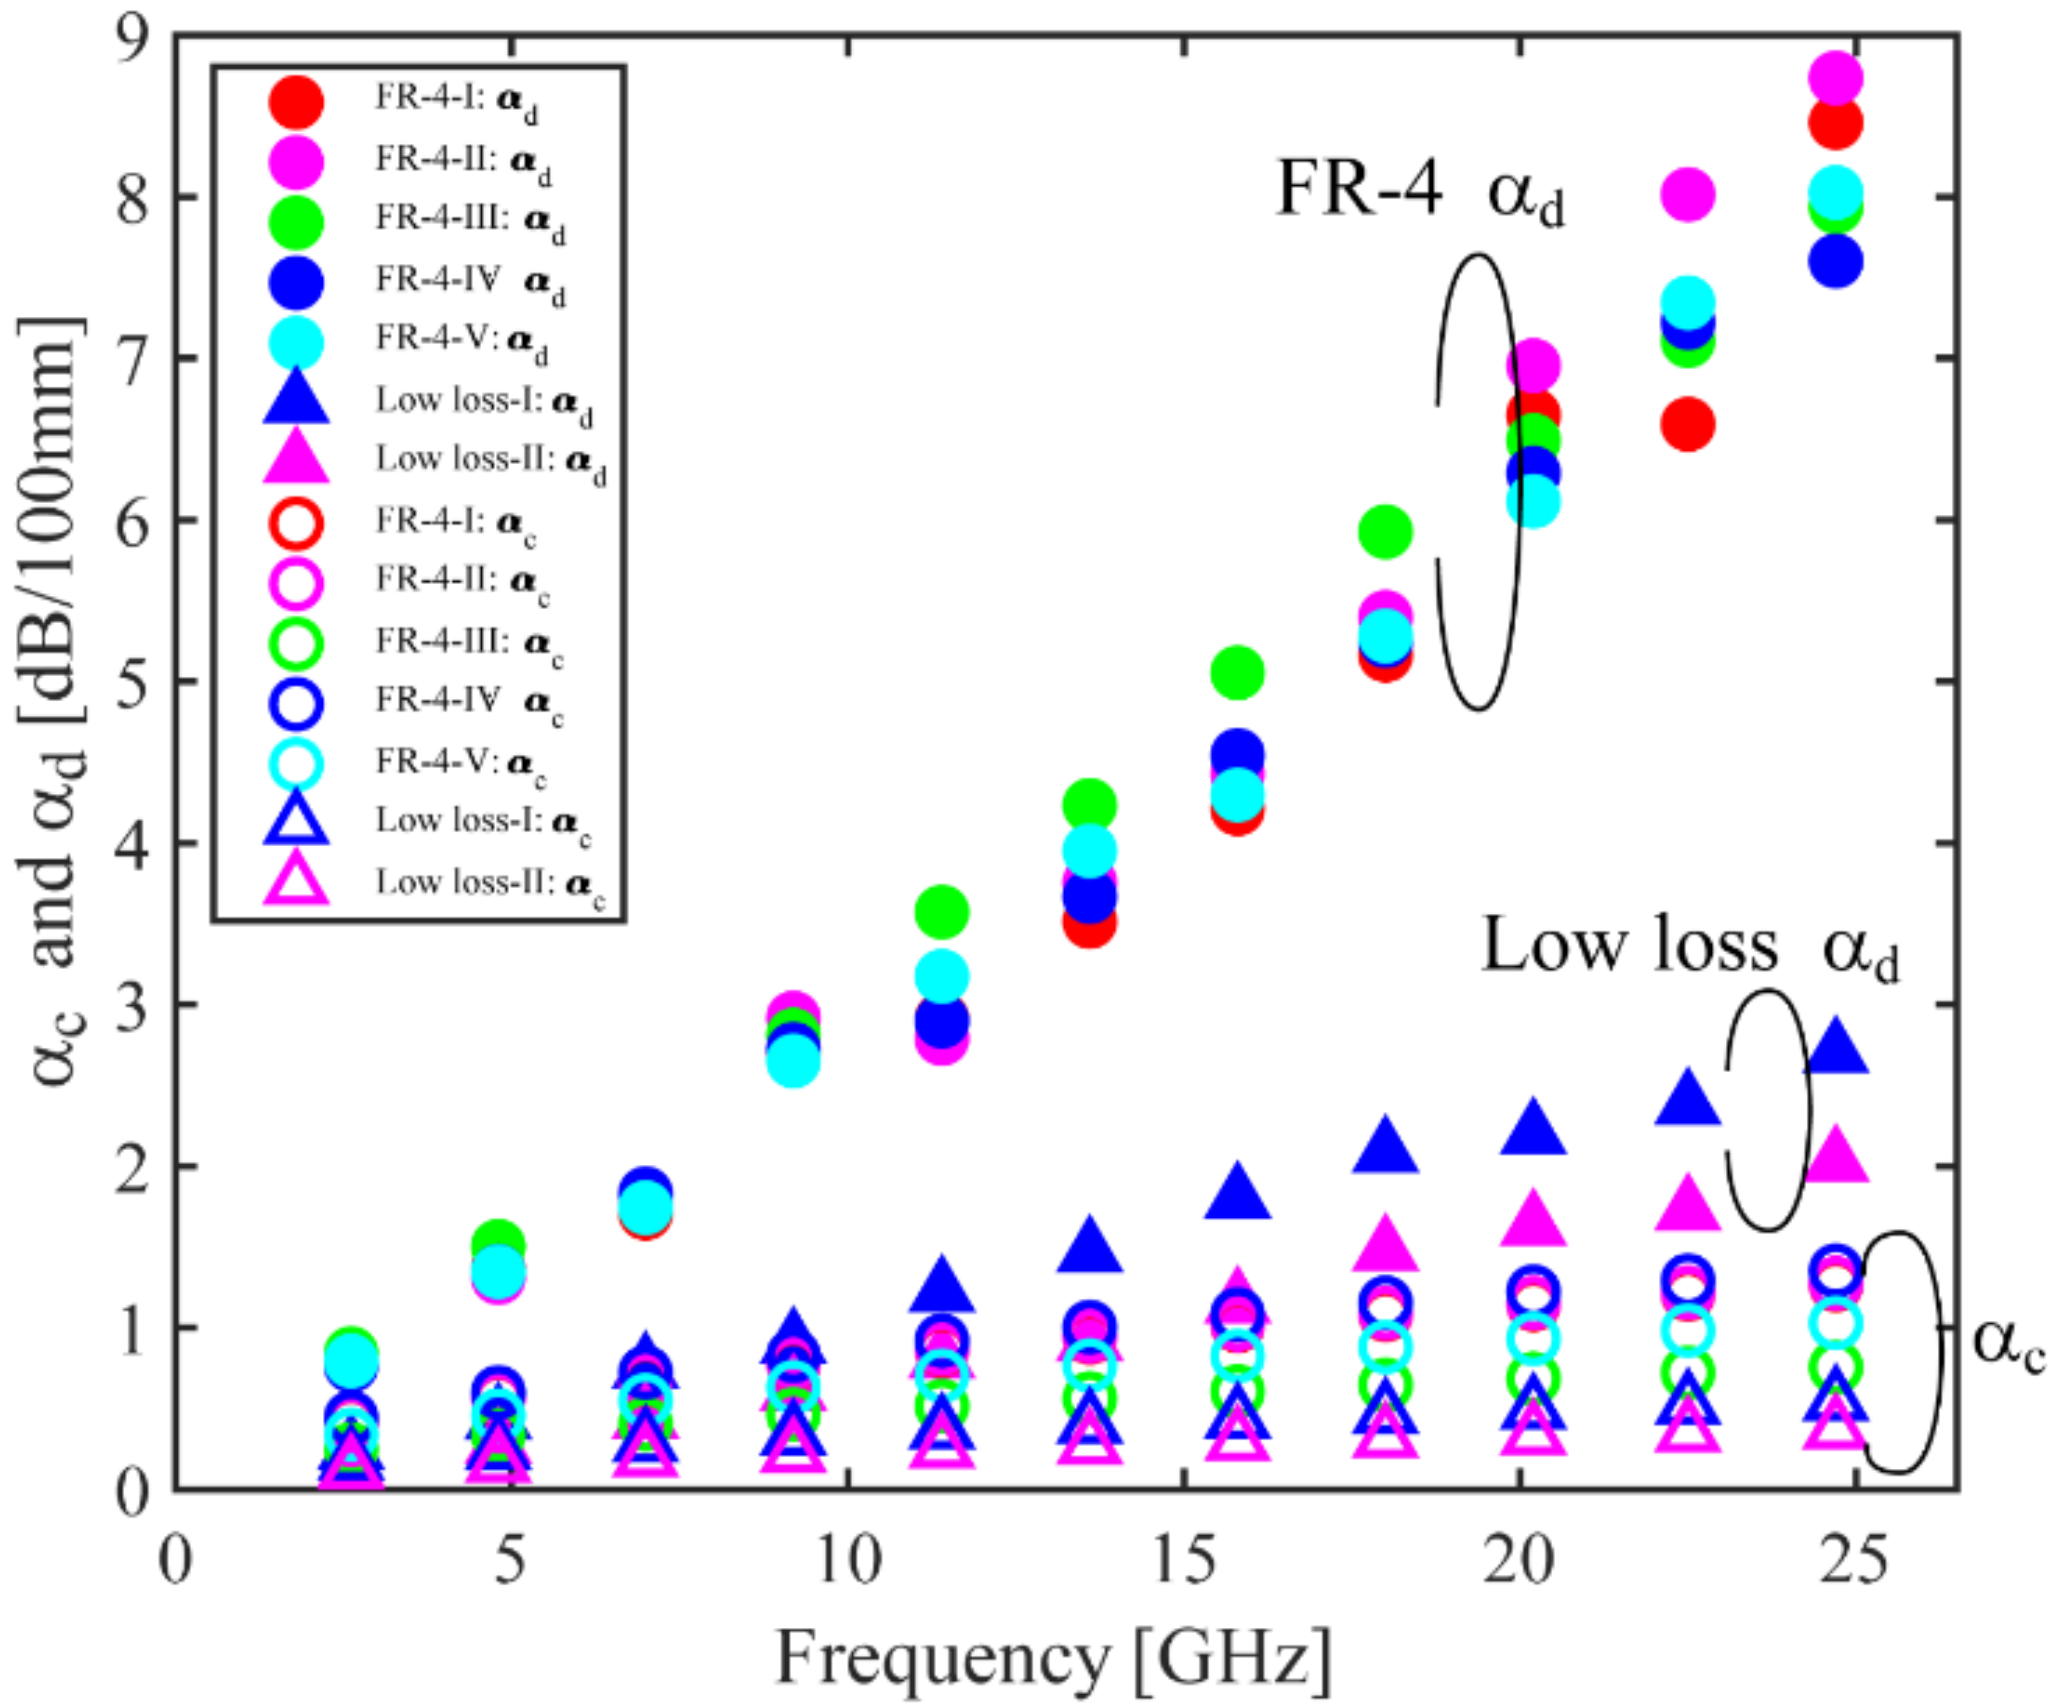
\includegraphics[width=0.8\textwidth]{input_file_0.png}
    \caption{各種基板材料における導体損失($\alpha_c$)と誘電損失($\alpha_d$)の周波数依存性.丸印がFR-4,三角印が低損失材料を示す.}
    \label{fig:loss_vs_freq}
\end{figure}

このグラフから,「高周波帯では誘電損失が支配的になる」という重要な結論が導かれます.例えばFR-4(丸印)を見ると,25 GHzでは誘電損失 $\alpha_d$(約 \SI{7.5}{\deci\bel/100mm})が,導体損失 $\alpha_c$(約 \SI{1.5}{\deci\bel/100mm})を遥かに上回っていることが一目瞭然です.

\section{界面効果と実効的導電率}
損失分離において,導体損失 $\alpha_c$ の理論計算は「バルクの導電率 $\sigma$」を用いて行われます.しかし,ミリ波のような極めて高い周波数帯では,銅箔の「表面」と「界面」の状態が無視できない影響を及ぼします.

\begin{itemize}
    \item \textbf{表面粗さの影響の再考}:
    第2章で述べた通り,表面粗さは電流経路を長くし,損失を増大させます.この効果をシミュレーションモデルに組み込む際,例えばHurayモデルやGroisseモデルが用いられます.これらのモデルは,実効的に「見かけの導電率」を低下させる,あるいは表面インピーダンスを増加させる形で損失増大を表現します.
    
    \item \textbf{界面の化学的影響}:
    基板製造プロセスにおいて,銅箔と誘電体樹脂の接着強度を確保するため,銅箔表面には酸化処理やシランカップリング剤による化学処理が施されます.この数nmから数十nmの薄い「界面層」は,純粋な銅とも誘電体とも異なる,導電率が低く損失の大きい層です.
    ミリ波帯では表皮深さがサブミクロンオーダーにまで浅くなるため,電流がこの界面層を流れる割合が増加し,バルク導電率から予測されるよりも大きな損失が生じる原因となります.
\end{itemize}
したがって,超高周波領域での精密な損失モデリングは,単純なバルク導電率だけでなく,これらの界面効果を考慮した「実効的導電率」や界面インピーダンスの概念を導入する必要があります.

\section{FR-4の利用限界と材料選定の重要性}
図 \ref{fig:loss_vs_freq} は,汎用基板材料であるFR-4がどの周波数帯まで利用可能かの評価にも有用です.

FR-4(丸印)は,低周波域(\SI{5}{\giga\hertz}以下)では全損失が比較的小さく,コスト面の利点から多くのアプリケーションで採用されます.しかし,周波数が高くなるにつれて誘電損失 $\alpha_d$ が急激に増大し,\SI{20}{\giga\hertz}を超える領域では,10cmの伝送路だけで信号パワーが半分以下(\SI{-3}{\deci\bel}以上)になるほどの大きな損失を示します.

これに対し,低損失材料(三角印)は,$\alpha_d$ の絶対値と周波数に対する増加勾配の両方が劇的に小さく抑えられています.\SI{25}{\giga\hertz}においても,全損失はFR-4の半分以下です.

この比較から,「どの周波数帯まで利用できるか」は,そのシステムが許容できる「損失マージン」に依存しますが,数十Gbpsの高速デジタル伝送や\SI{20}{\giga\hertz}を超えるマイクロ波回路では,FR-4の使用は現実的ではなく,低損失材料の選定が伝送品質を確保する上で不可欠であることが明確に示されています.

\clearpage
% ===================================================================
\part{質疑応答への準備}
% ===================================================================

\chapter{想定問答集}
上記1〜9章の知識に基づき,あなたの研究発表\cite{Yanagihara2025}で教授から投げかけられそうな専門的で鋭い質問を10個想定し,それぞれに対する模範解答を作成します.

\begin{description}
    \item[Q1.] \textbf{なぜ単純な伝送線路法(TL法)ではなく,わざわざBCDRのような共振器法を用いるのですか?その本質的な利点は何ですか?}
    \item[A1.] はい.TL法は信号の減衰定数 $\alpha$ を直接測定しますが,今回測定対象としたMEGTRON6\cite{Yanagihara2025}のような超低損失材料では $\alpha$ が極めて小さく,VNAの測定誤差内で有意な減衰を得るには,非現実的な線路長が必要となります\cite{Optica:resonatorloss}.
    共振器法は,電磁界エネルギーをQ値倍に共振器内部に蓄積させ\cite{PhysicsLibreTexts:TEMresonances},材料の微小な損失($\tan\delta$)を,「共振ピークの鋭さ($Q=f_r/\Delta f$)」という,VNAで高精度に測定可能な周波数指標に高感度に変換します\cite{iMapsource:highfreqmeas}.この「損失の増幅効果」が,低損失材料の精密測定における共振器法の本質的な利点です.

    \item[Q2.] \textbf{導体表面の粗さ(Roughness)が損失を増やす物理的メカニズムを,表皮深さ(Skin Depth)と関連付けて説明してください.}
    \item[A2.] はい.高周波では表皮効果により電流が表面に集中し,その深さ $\delta_s$ は $1/\sqrt{f}$ に比例して浅くなります\cite{YouTube:SkinEffect}.周波数が高くなり,$\delta_s$ が銅箔の表面粗さ(数\si{\micro\meter})と同等以下になると,主に2つのメカニズムで損失が増大します\cite{ElectronicsOrg:2020}.
    第一に,電流が粗さの山谷の地形に沿って流れるため,実効的な電流経路長が平滑な場合より増大し,抵抗が増加します\cite{PolarInstruments:2025}.
    第二に,粗さの「谷」部分では,電流が谷底に集中し,両側の壁を流れる電流との近接効果によって局所的な磁界集中が発生します.この強まった磁界が,さらに強力な渦電流(損失)を誘導するためです.

    \item[Q3.] \textbf{あなたのBCDR測定系において,$\epsilon_r$ や $\tan\delta$ の測定精度を左右する,最大の誤差要因は何だと考えますか?}
    \item[A3.] エアギャップ(Air Gap),すなわちBCDRの導体板と測定サンプル(基板)との間に生じる,ミクロンレベルのわずかな隙間だと考えます\cite{IEEE:BCDR220GHz}.
    このエアギャップは,比誘電率が1で損失がゼロの微小なコンデンサが,サンプルと直列に接続されたかのような影響を与えます.これにより,特にMEGTRON6のような高誘電率・低損失材料では,測定される実効的な $\epsilon_r$ と $\tan\delta$ は,真の値よりも著しく低く見積もられてしまいます\cite{IEEE:BCDR220GHz}.測定時には,このギャップを最小化するよう,均一な圧力を加える機構が重要になります.

    \item[Q4.] \textbf{発表スライド9ページ\cite{Yanagihara2025}では,高周波側で共振ピークの形が崩れていますが,これはなぜですか?なぜそのデータを計算から除外したのですか?}
    \item[A4.] ご指摘の通り,高周波領域でピークのQ値が低下し,形状が崩れています.これは,MEGTRON6の材料特性が劣化したのではなく,測定系(BCDR)の限界によるものだと考えています.
    具体的には,(1)目的の TM\textsubscript{0m0} モード\cite{IEEE:BCDR220GHz}以外の,TEモードやハイブリッドモードといった不要なスプリアス共振が発生し,目的のモードと干渉(モードカップリング)を起こしている可能性,(2)周波数が高くなり波長が短くなったことで,共振器の側面(開放端)からの放射損失が無視できなくなった可能性,が考えられます.
    これらの不要な損失要因が含まれたデータでは,材料本来の $\tan\delta$ を正確に分離・算出することができません.そのため,ピーク形状が理論通り明確で,不要な損失の影響が小さいと判断できる周波数帯のデータのみを使用しました\cite{Yanagihara2025}.

    \item[Q5.] \textbf{損失の分離式\cite{Yanagihara2025}は $1/Q = 1/Q_c + 1/Q_d$ と「逆数の和」で表されます.なぜQそのものの和 $Q = Q_c + Q_d$ ではないのですか?}
    \item[A5.] それは,Q値の物理的定義 $Q = \omega W_{\mathrm{stored}} / P_{\mathrm{loss}}$\cite{UltrasonicResonators:Qfactor}と,物理法則である「電力の加法性」に基づいています\cite{ElectricalTechnology:Qfactor}.
    共振器全体の消費電力 $P_{\mathrm{total}}$ は,導体損失 $P_c$ と誘電損失 $P_d$ の単純な和で表されます($P_{\mathrm{total}} = P_c + P_d$).
    この式の両辺を,系に蓄積されるエネルギー $\omega W_{\mathrm{stored}}$ で割ると,$P_{\mathrm{loss}} / (\omega W_{\mathrm{stored}})$ という項は $1/Q$ と定義されます\cite{EngLibreTexts:Qfactor_fund}.
    したがって,$1/Q_{\mathrm{total}} = 1/Q_c + 1/Q_d$ となり,「$1/Q$(規格化された損失率)」が,消費電力と同様の加法性を持つためです.

    \item[Q6.] \textbf{あなたの研究の最終目的は「表面粗さの影響」を調べること\cite{Yanagihara2025}ですが,今回の発表では「まず誘電損失を測定」しています.この論理的な繋がりを説明してください.}
    \item[A6.] はい.最終的に知りたいのは,表面粗さを含む導体損失 $Q_c$ です.しかし,VNAで測定できるのは全体の損失 $Q_0$ だけであり,損失分離式 $1/Q_0 = 1/Q_c + 1/Q_d$ には $Q_c$ と $Q_d$ という2つの未知数が含まれます.
    そこで,この問題を解決するために,2段階の測定戦略をとります.
    \textbf{第1段階}が今回の発表内容で,表面が極めて平滑な「標準銅箔」と誘電体コア材で基準共振器を構成し,表面粗さの影響を完全に排除した状態で,材料固有の真の誘電損失 $Q_d$(すなわち $\tan\delta$)を精密に決定します.
    \textbf{第2段階}として,その既知となった $Q_d$ を利用して,本当に評価したい「粗さのある基板」の全体の損失 $Q_0$ から $1/Q_c = 1/Q_0 - 1/Q_d$ の関係を用いて,表面粗さの影響を含んだ真の導体損失 $Q_c$ を正確に分離します.
    このように,まず $\tan\delta$ を確定させることが,最終目的である導体損失評価の論理的な前提となるためです.

    \item[Q7.] \textbf{BCDR法では TM\textsubscript{0m0} モードを利用するとのことですが,このモードが誘電体シートの測定に適しているのはなぜですか?}
    \item[A7.] TM\textsubscript{0m0} モードは,その電磁界分布に特徴があります.電界 $E$ が基板に対して垂直な成分($E_z$)のみを持ち,磁界 $H$ が同心円状の成分($H_\phi$)のみを持つ,非常にシンプルな円筒対称のモードです\cite{ScholarsMine:TM010}.
    基板材料の $\epsilon_r$ や $\tan\delta$ は,主に電界によって決まる物性です.$E_z$ が基板全面に一様に印加されるこのモードは,基板の $z$ 方向(厚さ方向)の誘電特性を測定する上で,最も理想的かつ解析しやすい電磁界分布であるため,BCDR法で選択的に利用されます\cite{IEEE:BCDR220GHz}.
    
    \item[Q8.] \textbf{複素誘電率 $\epsilon = \epsilon' - \mi\epsilon''$ の「虚数部 $\epsilon''$」とは,物理的に何を意味しますか?}
    \item[A8.] 複素誘電率は,物質に印加した時間変化する電界 $E$ と,それに対する物質の応答(電束密度 $D$)の間の「位相の遅れ」を表現したものです\cite{VTechWorks:diel_perf}.
    実数部 $\epsilon'$ は電界と同位相の応答で,エネルギーを「蓄積」する能力($\epsilon_r$)を意味します\cite{Microwaves101:permittivity}.
    虚数部 $\epsilon''$ は電界と90°遅れた応答で,分極が電界に追従しきれない\cite{wiki:dielectric}ことによる「摩擦」や「抵抗」を意味し,1サイクルあたりに熱として「損失」されるエネルギーの大きさを表します\cite{Microwaves101:permittivity}.

    \item[Q9.] \textbf{減衰定数 $\alpha$ と Q値 の関係式 $\alpha = \beta / (2Q)$ を導出する際,「群速度 $v_g$」と「位相速度 $v_p$」がどのように関わってくるのか説明してください.}
    \item[A9.] はい.この式の厳密な導出は,Qのエネルギー定義 $Q = \omega W'_{\mathrm{stored}} / P'_{\mathrm{loss}}$ から始まります.ここで,電力 $P$ はエネルギーが伝わる速度,すなわち群速度 $v_g$ で蓄積エネルギー $W'_{\mathrm{stored}}$ を運ぶため,$P = W'_{\mathrm{stored}} \times v_g$ と表されます\cite{IEEE:alphaQrelation}.
    これらを整理すると,厳密な関係式 $\alpha = \omega / (2 Q v_g)$ が得られます.ここで $v_g = \dd\omega / \dd\beta$ です\cite{Testbook:group_phase}.
    一方,位相速度は $v_p = \omega / \beta$ です\cite{Testbook:group_phase}.もし媒質が「無分散」で $v_g = v_p$ と近似できる場合にのみ\cite{EngLibreTexts:TLT},$\alpha = \omega / (2Q (\omega/\beta))$ となり,ご質問の $\alpha = \beta / (2Q)$ という簡略化された関係式が導出されます.

    \item[Q10.] \textbf{VNAはどのようにしてSパラメータの「位相」を測定しているのですか? ギガヘルツの波の位相を直接測るのは困難ではないですか?}
    \item[A10.] 非常に良いご質問です.VNAはギガヘルツの位相を\textbf{直接}測定しているわけではありません.\textbf{ヘテロダイン検波}という原理を用いています\cite{AllAboutCircuits:VNA}.
    \begin{enumerate}
        \item まず,VNAは基準信号 $a_1$ を「R受信機」で,透過信号 $b_2$ を「T受信機」で受けます\cite{Keysight:VNA}.
        \item VNA内部の局部発振器(LO)とこれら2つの信号を「混合(Mix)」します.
        \item これにより,両方の受信機で,例えば数\si{\mega\hertz}の非常に低い\textbf{中間周波数(IF)}の信号が生成されます\cite{NI:VNA}.
        \item 重要なのは,このIF信号が,元のギガヘルツ信号の「振幅情報」と「位相情報」を\textbf{そのまま保持している}ことです.
        \item VNAは,この測定しやすいIF信号の「R受信機のIF位相」と「T受信機のIF位相」の\textbf{位相差}をデジタル的に精密測定します.これが $\angle S_{21}$ となります.
    \end{enumerate}
    つまり,ギガヘルツの位相差を,測定可能なIF周波数の位相差に「変換」して測定しています.
\end{description}

\clearpage
\begin{sloppypar}
\emergencystretch=4em
\begin{thebibliography}{99}
    \bibitem{Yanagihara2025} 5中間発表\_柳原.pdf
    \bibitem{wiki:dielectric} Dielectric - Wikipedia, accessed Nov. 13, 2025, \url{https://en.wikipedia.org/wiki/Dielectric}
    \bibitem{VTechWorks:diel_perf} Chapter 5 Dielectric Performance - VTechWorks, accessed Nov. 13, 2025, \url{https://vtechworks.lib.vt.edu/bitstream/handle/10919/40359/ch5.pdf}
    \bibitem{ACSPublications:2014} Exploring Strategies for High Dielectric Constant and Low Loss Polymer Dielectrics | The Journal of Physical Chemistry Letters - ACS Publications, accessed Nov. 13, 2025, \url{https://pubs.acs.org/doi/10.1021/jz501831q}
    \bibitem{EnergySustainabilityDirectory:2025} Dielectric Polarization Mechanisms → Term - Energy → Sustainability Directory, accessed Nov. 13, 2025, \url{https://energy.sustainability-directory.com/term/dielectric-polarization-mechanisms/}
    \bibitem{wiki:permittivity} Permittivity - Wikipedia, accessed Nov. 13, 2025, \url{https://en.wikipedia.org/wiki/Permittivity}
    \bibitem{Microwaves101:permittivity} Microwaves101 | Permittivity - Microwave Encyclopedia, accessed Nov. 13, 2025, \url{https://www.microwaves101.com/encyclopedias/permittivity}
    \bibitem{YouTube:ComplexPermittivity} Defining Complex Permittivity - YouTube, accessed Nov. 13, 2025, \url{https://www.youtube.com/watch?v=pswL_Ce8ooE}
    \bibitem{Altium:2025} The Increasingly Important Role of Loss Tangents in PCB Laminates, accessed Nov. 13, 2025, \url{https://resources.altium.com/p/increasingly-important-role-loss-tangents-pcb-laminates}
    \bibitem{OilTester:TanDelta} Tan Delta dielectric loss tangent angle definition, detection significance - Oil-tester.com, accessed Nov. 13, 2025, \url{https://www.oil-tester.com/tan-delta-dielectric-loss-tangent-angle-definition-detection-significance/}
    \bibitem{HVI:2019} TAN δ CABLE TESTING Overview \& Answers to Frequently Asked Questions - High Voltage Inc, accessed Nov. 13, 2025, \url{https://hvinc.com/wp-content/uploads/2019/11/HVI-TD-FAQ-WEB-2019.pdf}
    \bibitem{MDPI:2023} Applied Sciences | Free Full-Text | Analytical Calculation of the ..., accessed Nov. 13, 2025, \url{https://www.mdpi.com/2076-3417/13/22/12416}
    \bibitem{AIFutureSchool:2025} Understanding the Skin Effect in High Frequency Conductors - AI-FutureSchool, accessed Nov. 13, 2025, \url{https://www.ai-futureschool.com/en/electrotechnics/understanding-skin-effect-in-high-frequency-conductors.php}
    \bibitem{InComplianceMagazine:2025} Skin Depth in Good Conductors - In Compliance Magazine, accessed Nov. 13, 2025, \url{https://incompliancemag.com/skin-depth-in-good-conductors/}
    \bibitem{YouTube:SkinEffect} Skin Effect and Skin Depth Explained: Basics, Derivation, and Parameters - YouTube, accessed Nov. 13, 2025, \url{https://www.youtube.com/watch?v=xJvYwZb5Bvk}
    \bibitem{ElectronicsOrg:2020} Effect of Conductor Surface Roughness upon Measured Loss and Extracted Values of PCB Laminate Material Dissipation Factor, accessed Nov. 13, 2025, \url{https://www.electronics.org/system/files/technical_resource/E8%26S20_02.pdf}
    \bibitem{PolarInstruments:2025} Surface roughness effect on PCB trace attenuation / loss by Hammerstad Groisse and Huray snowball method - Polar Instruments, accessed Nov. 13, 2025, \url{https://www.polarinstruments.com/support/si/AP8155.html}
    \bibitem{Ansys:Sparam} What Are S-parameters? - Ansys, accessed Nov. 13, 2025, \url{https://www.ansys.com/simulation-topics/what-are-s-parameters}
    \bibitem{SierraCircuits:Sparam} S-parameters Measurement Using VNA | Sierra Circuits, accessed Nov. 13, 2025, \url{https://www.protoexpress.com/blog/s-parameters-measurement-vector-network-analyzer/}
    \bibitem{Coilcraft:Sparam} S-Parameters for High Frequency Circuit Simulation | Coilcraft, accessed Nov. 13, 2025, \url{https://www.coilcraft.com/en-us/resources/application-notes/s-parameters-for-high-frequency-circuit-simulation/}
    \bibitem{wiki:Sparam} Scattering parameters - Wikipedia, accessed Nov. 13, 2025, \url{https://en.wikipedia.org/wiki/Scattering_parameters}
    \bibitem{Keysight:VNA} VNA FAQ: An Introduction | Keysight Blogs, accessed Nov. 13, 2025, \url{https://www.keysight.com/blogs/en/tech/rfmw/2023/03/02/vna-faq-an-introduction}
    \bibitem{AllAboutCircuits:VNA} Understanding the Inner Workings of Vector Network Analyzers - Technical Articles, accessed Nov. 13, 2025, \url{https://www.allaboutcircuits.com/technical-articles/the-inner-workings-of-vector-network-analyzers-exploring-the-signal-source-and-receivers/}
    \bibitem{NI:VNA} Introduction to Network Analyzer Measurements - ni, accessed Nov. 13, 2025, \url{http://download.ni.com/evaluation/rf/Introduction_to_Network_Analyzer_Measurements.pdf}
    \bibitem{Anritsu:VNA} Understanding Vector Network Analysis Product Guide, accessed Nov. 13, 2025, \url{https://dl.cdn-anritsu.com/en-us/test-measurement/files/Application-Notes/Application-Note/11410-00724D.pdf}
    \bibitem{Warwick:resonator} Resonators - University of Warwick, accessed Nov. 13, 2025, \url{https://warwick.ac.uk/fac/sci/physics/research/condensedmatt/imr_cdt/students/stephen_hogg/resonators/}
    \bibitem{PhysicsStackExchange:EMresonance} Can there be resonance in electromagnetic waves? - Physics Stack Exchange, accessed Nov. 13, 2025, \url{https://physics.stackexchange.com/questions/354743/can-there-be-resonance-in-electromagnetic-waves}
    \bibitem{MIT:ResonantCavities} Resonant Cavities and Waveguides - MIT, accessed Nov. 13, 2025, \url{https://web.mit.edu/22.09/ClassHandouts/Charged%20Particle%20Accel/CHAP12.PDF}
    \bibitem{TaylorFrancis:Qfactor} Q factor | Definition, Equation, \& Facts | Britannica, accessed Nov. 13, 2025, \url{https://www.britannica.com/technology/Q-factor}
    \bibitem{wiki:Qfactor} Q factor - Wikipedia, accessed Nov. 13, 2025, \url{https://en.wikipedia.org/wiki/Q_factor}
    \bibitem{Fiveable:Qfactor} Quality factor and bandwidth | Electrical Circuits and Systems II Class Notes - Fiveable, accessed Nov. 13, 2025, \url{https://fiveable.me/electrical-circuits-systems-ii/unit-4/quality-factor-bandwidth/study-guide/75pXRlt90vyTwa7w}
    \bibitem{PMC:SuperDamping} Super Damping of Mechanical Vibrations - PMC - PubMed Central, accessed Nov. 13, 2025, \url{https://pmc.ncbi.nlm.nih.gov/articles/PMC6882872/}
    \bibitem{IEEE:BCDR220GHz} Broadband Perpendicular Permittivity Measurements up to 220 GHz Using a Balanced-Type Circular Disk Resonator Without - IEEE Xplore, accessed Nov. 13, 2025, \url{https://ieeexplore.ieee.org/iel8/19/4407674/11006707.pdf}
    \bibitem{ResearchGate:BCDRanalysis} \href{https://www.researchgate.net/publication/3937129}{Analysis of Balanced-Type Circular Disk Resonator}, accessed Nov. 13, 2025
    \bibitem{ScholarsMine:TM010} Design of the TM010 Mode Cylindrical Cavity Resonator for PCB Dielectric Characterization - Scholars' Mine, accessed Nov. 13, 2025, \url{https://scholarsmine.mst.edu/cgi/viewcontent.cgi?article=7814&context=ele_comeng_facwork}
    \bibitem{Panasonic:diel_loss} On dielectric constant and loss tangent of dielectric material for circuit boards, accessed Nov. 13, 2025, \url{https://industrial.panasonic.com/content/data/EM/PDF/2021_5G_Multilayer_PCB_Solutions_WhitePaper_202108.pdf}
    \bibitem{Intel:losstangent} 1.2.1.2. Loss Tangent - Intel, accessed Nov. 13, 2025, \url{https://www.intel.com/content/www/us/en/docs/programmable/683883/current/loss-tangent.html}
    \bibitem{Optica:resonatorloss} Modeling and measurement of losses in silicon-on-insulator resonators and bends, accessed Nov. 13, 2025, \url{https://opg.optica.org/oe/abstract.cfm?uri=oe-15-17-10553}
    \bibitem{PhysicsLibreTexts:TEMresonances} 7.4: TEM Resonances - Physics LibreTexts, accessed Nov. 13, 2025, \url{https://phys.libretexts.org/Bookshelves/Electricity_and_Magnetism/Electromagnetics_and_Applications_(Staelin)/07:_TEM_transmission_lines/7.04:_TEM_resonances}
    \bibitem{iMapsource:highfreqmeas} Optimizing Measurement Accuracy and Repeatability for High Frequency Measurements, accessed Nov. 13, 2025, \href{https://imapsource.org/api/v1/articles/116510-optimizing-measurement-accuracy-and-repeatability-for-high-frequency-measurements.pdf}{iMapsource Link}
    \bibitem{CMT:Qfactor} Determining Resonator Q Factor from Return Loss Measurement Alone, accessed Nov. 13, 2025, \url{https://coppermountaintech.com/determining-resonator-q-factor-from-return-loss-measurement-alone/}
    \bibitem{ECStudio:Qfactor} Quality Factor and Bandwidth - Filters - Basics Electronics - electric circuit studio, accessed Nov. 13, 2025, \url{https://ecstudiosystems.com/discover/textbooks/basic-electronics/filters/quality-factor-and-bandwidth/}
    \bibitem{Hapislab:TanDel} 複素誘電率, accessed Nov. 13, 2025, \url{https://hapislab.org/public/makino/materials/20071030_TanDel.pdf}
    \bibitem{UltrasonicResonators:Qfactor} Quality factor (Q) (definition) - Ultrasonic Resonators, accessed Nov. 13, 2025, \url{https://www.ultrasonic-resonators.org/glossary/q1_dict.html}
    \bibitem{IEEE:alphaQrelation} On "A relation between α and Q" | IEEE Journals \& Magazine, accessed Nov. 13, 2025, \url{https://ieeexplore.ieee.org/document/1443802/1000}
    \bibitem{Testbook:group_phase} Relation Between Group Velocity and Phase Velocity - Testbook, accessed Nov. 13, 2025, \url{https://testbook.com/physics/relation-between-group-velocity-and-phase-velocity}
    \bibitem{EngLibreTexts:TLT} 2.2: Transmission Line Theory - Engineering LibreTexts, accessed Nov. 13, 2025, \url{https://eng.libretexts.org/Bookshelves/Electrical_Engineering/Electronics/Microwave_and_RF_Design_II_-_Transmission_Lines_(Steer)/02:_Transmission_Lines/2.02:_Transmission_Line_Theory}
    \bibitem{ElectricalTechnology:Qfactor} Q Factor in Electrical and Electronics Engineering, accessed Nov. 13, 2025, \url{https://www.electricaltechnology.org/2013/11/q-factor-in-electrical-and-electronics-engineering.html}
    \bibitem{EngLibreTexts:Qfactor_fund} 9.2: Q Factor - Engineering LibreTexts, accessed Nov. 13, 2025, \url{https://eng.libretexts.org/Bookshelves/Electrical_Engineering/Electronics/Book:_Fundamentals_of_Microwave_and_RF_Design_(Steer)/09:_Passive_Components/9.02:_Q_Factor}
\end{thebibliography}
\end{sloppypar}

\end{document}